\documentclass[10pt,a4paper]{article}
\usepackage[margin=22mm]{geometry}\usepackage[T1]{fontenc}\usepackage{lmodern,microtype,booktabs,graphicx,xcolor,hyperref,tcolorbox,parskip}
\definecolor{ink}{HTML}{172B4D}\definecolor{teal}{HTML}{137C8B}\definecolor{mist}{HTML}{F1F6F8}
\hypersetup{colorlinks=true,linkcolor=teal,urlcolor=teal}
\title{\vspace{-2em}\color{ink}\bfseries NOAA block-length sensitivity\\[-.2em]\large Reference and correctness-calibrator uncertainty}
\author{Phase 3 natural-stream addendum}\date{17 November 2026}
\begin{document}\maketitle\vspace{-1em}
\begin{tcolorbox}[colback=mist,colframe=teal,boxrule=0pt,leftrule=2mm]\textbf{Scope.} One station, one chronological same-day classification holdout. The classifier is fixed. These resampling diagnostics are conditional sensitivity summaries, not population guarantees.
\end{tcolorbox}
\section*{Design}
We repeated the same 200-replicate calibrator-only, reference-only and joint moving-block bootstrap with block lengths of 7, 30 and 90 consecutive daily rows. The 30-day run is the primary diagnostic; 7 and 90 days test dependence-length sensitivity. Each run resamples calibration confidence/correctness pairs and reference correctness, then exactly recomputes the plug-in Poisson-binomial concern score for the same 21 monitor batches. Model-fit uncertainty is not resampled. Monitor outcomes are evaluator-only.
\section*{Result}
Under joint resampling, the average per-batch 95\% accuracy-estimate interval width increased from 0.037 at 7 days, to 0.045 at 30 days, and 0.059 at 90 days. Expected-harm concern interval widths were 0.184, 0.219 and 0.259, respectively. The average fraction of bootstrap concern flags disagreeing with the original plug-in decision was 0.003, 0.007 and 0.010. Longer blocks produce wider uncertainty intervals and somewhat more decision disagreement in this selected diagnostic, so uncertainty depends on the temporal resampling scale.
\begin{center}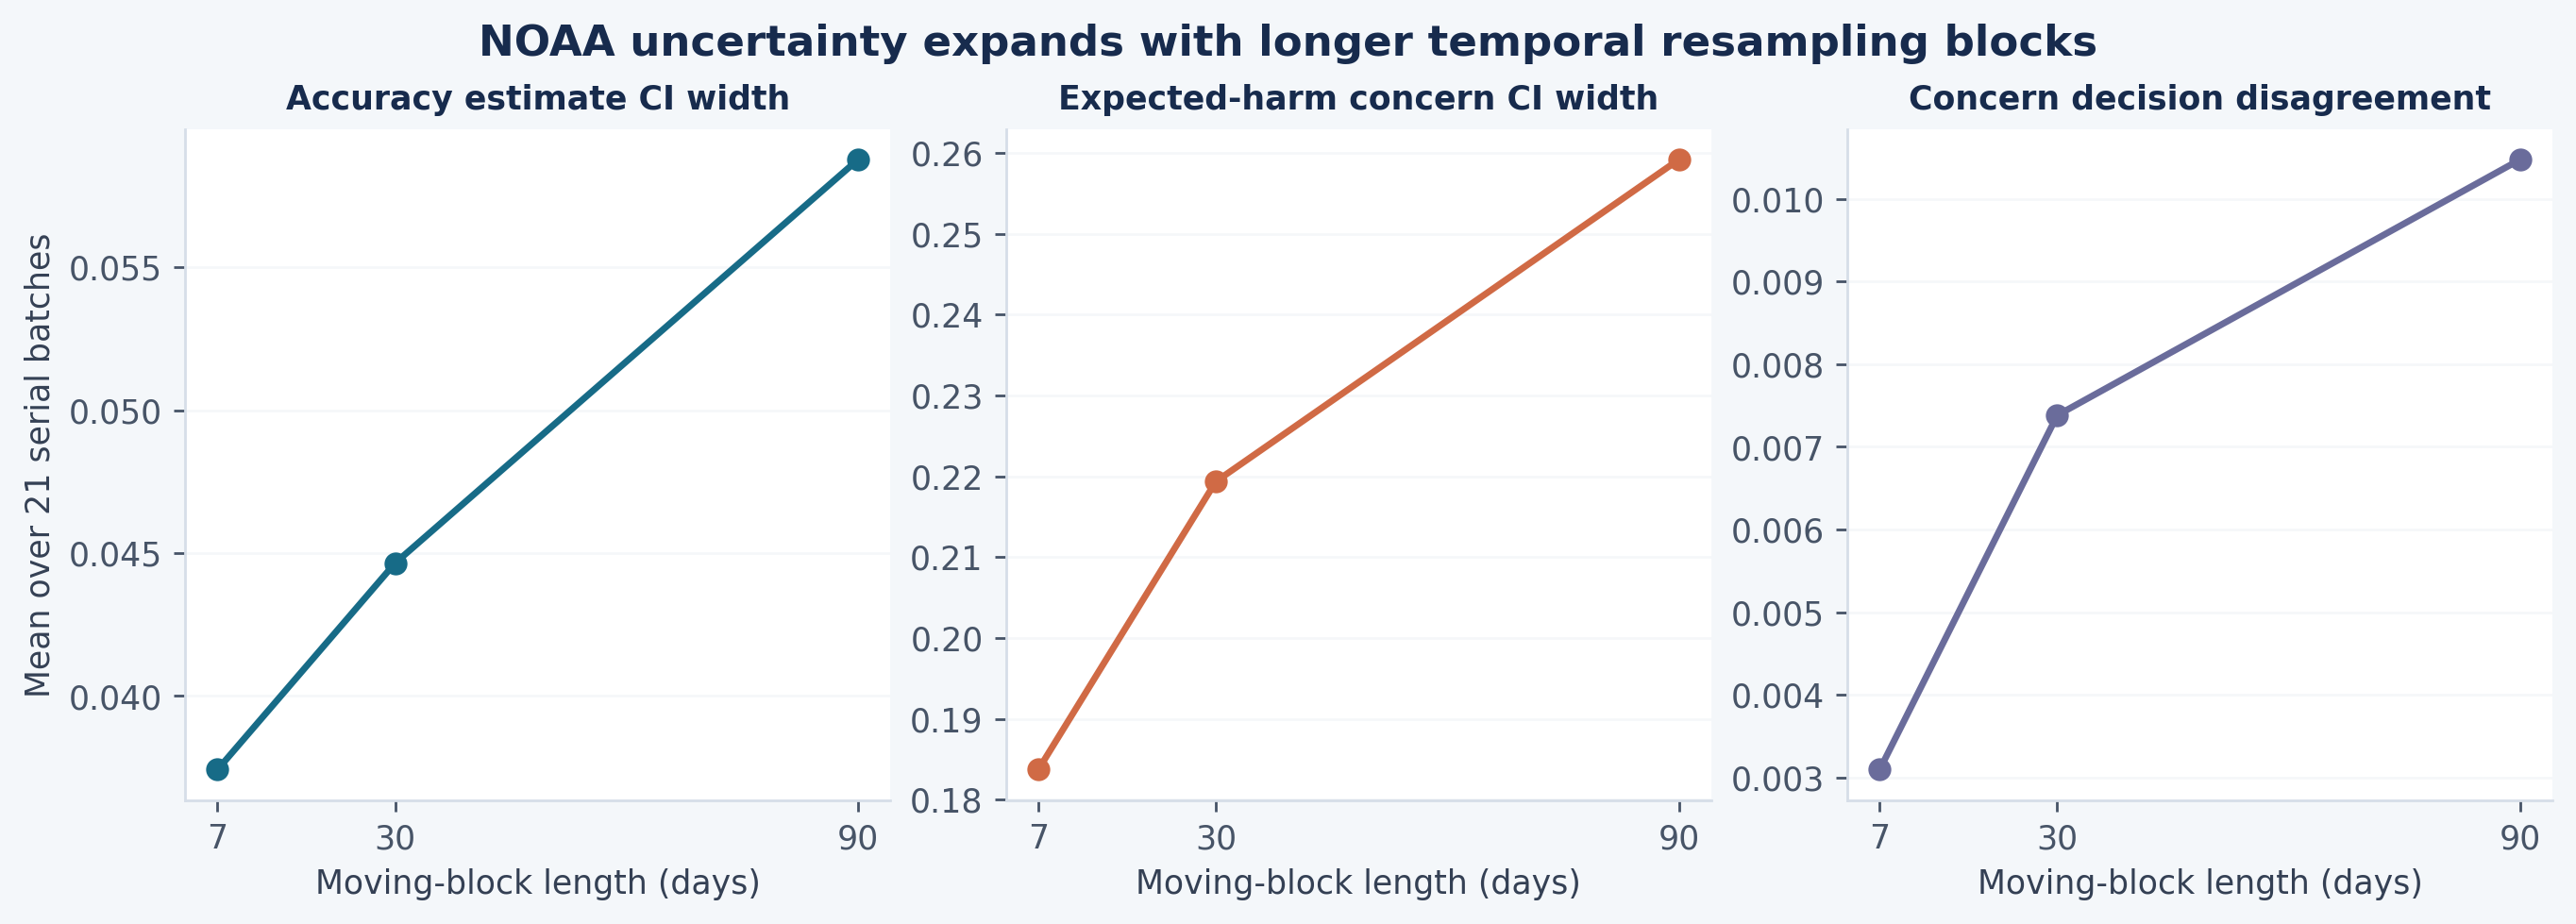
\includegraphics[width=\linewidth]{block_length_sensitivity.png}\end{center}
\section*{Interpretation}
This sensitivity checks a single station's calibration/reference partitions under three block lengths; it does not identify the true dependence horizon. The 90-day scheme has relatively few effective blocks in these historical segments; 7-day blocks may understate longer dependence. Report the 30-day analysis as a transparent reference choice, and include this spread as a limitation. The result does not account for fitting uncertainty in the logistic classifier, alternative stations, other temporal splits, or distribution-free coverage.
\section*{Reproduction}
Run the three block-bootstrap commands recorded in the accompanying audit receipts, then run \texttt{scripts/summarize\_noaa\_block\_length\_sensitivity.py}. Full per-draw CSVs and checksums are included.
\end{document}
